\documentclass[runningheads]{llncs}


\usepackage{subcaption}
\usepackage{graphicx}
\usepackage{tikz}

\begin{document}

\title{Planare Graphen - Coloring}
\author{Manuel Frohn}
\institute{RWTH Aachen University, Aachen, Germany\\
\email{manuel.frohn@rwth-aachen.de}}

\maketitle

\begin{abstract}
Die Klasse der Planaren Graphen ist sowol für die innermathematische Untersuchung von Graphen, als auch zur Modelierung
praktischer Netzwerke, wie zum Beispiel Straßennetze, oder Landkarten wichtig. So dient die Planarität von Graphen als 
Bedingung für die Funktionalität und/oder Effizienz einiger Algorithmen. Zu diesen zählt auch der Algorithmus zur 
Berechnung einer  4-Färbung in polinomieller Zeit. Die Berechnung einer Färbung ist ein Problem das viele Anwendungen
findet. Es lassen sich unter anderem viele Zuweisungsprobleme wie zum Beispiel Stundenplanerstellung oder auch 
Speicherzuweisung als Coloring Problem modelieren. 

\keywords{Planare Graphen \and Coloring}
\end{abstract}

\newpage

\section{Planare Graphen}
\subsection{Einführung}
%planar hervorheben
\begin{definition}[Planarität]
    Ein Graph G heißt planar, wenn man in der Lage ist, den Graphen so auf eine Ebene zu zeichnen, dass sich seine 
    Kanten nicht schneiden.
\end{definition}
Planare Graphen sind unter anderem durch die sehr graphische Natur ihrere Definition, eine Graphklasse, die schon sehr
lange untersucht wird. Um ein besseres Verständnis für die Graphklasse zu entwickeln wollen wir uns nun folgende Abbildungen
anschauen.

\begin{figure}
    \begin{subfigure}{.33\textwidth}
        \centering
        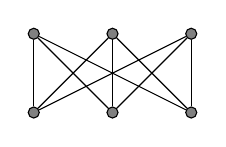
\begin{tikzpicture}[every node/.style={circle, draw, fill=black!50,inner sep=0pt, minimum width=4pt},
            edge_style/.style={draw=black}]
            \node (v1) at (0, 0) {};
            \node (v2) at (1, 0) {};
            \node (v3) at (2, 0) {};
            \node (v4) at (0, 1) {};
            \node (v5) at (1, 1) {};
            \node (v6) at (2, 1) {};  
            \draw (v1) edge (v4);
            \draw (v1) edge (v5);
            \draw (v1) edge (v6);
            \draw (v2) edge (v4);
            \draw (v2) edge (v5);
            \draw (v2) edge (v6);
            \draw (v3) edge (v4);
            \draw (v3) edge (v5);
            \draw (v3) edge (v6);
        \end{tikzpicture}
        \caption{}
    \end{subfigure}
    \begin{subfigure}{.33\textwidth}
        \centering
        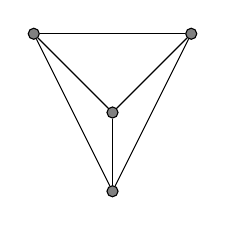
\begin{tikzpicture}[every node/.style={circle, draw, fill=black!50,inner sep=0pt, minimum width=4pt},
            edge_style/.style={draw=black}]
            \node (v1) at (1, 0) {};
            \node (v2) at (1, 1) {};
            \node (v3) at (0, 2) {};
            \node (v4) at (2, 2) {};
            \draw (v1) edge (v2);
            \draw (v1) edge (v3);
            \draw (v1) edge (v4);
            \draw (v2) edge (v3);
            \draw (v2) edge (v4);
            \draw (v4) edge (v3);
        \end{tikzpicture}
        \caption{}
    \end{subfigure}
    \begin{subfigure}{.32\textwidth}
        \centering
        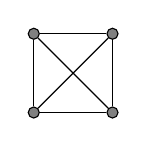
\begin{tikzpicture}[every node/.style={circle, draw, fill=black!50,inner sep=0pt, minimum width=4pt},
            edge_style/.style={draw=black}]
            \node (v1) at (0, 0) {};
            \node (v2) at (0, 1) {};
            \node (v3) at (1, 0) {};
            \node (v4) at (1, 1) {};
            \draw (v1) edge (v2);
            \draw (v1) edge (v3);
            \draw (v1) edge (v4);
            \draw (v2) edge (v3);
            \draw (v2) edge (v4);
            \draw (v4) edge (v3);
        \end{tikzpicture}
        \caption{}
    \end{subfigure}
    \caption{Der $ K_{3,3} $ (a) ist nicht planar, der $ K_4 $ (b) jedoch schon, lässt sich aber trozdem mit 
    Kantenüberschneidung zeichnen (c)}
\end{figure}


(a) zeigt den sogenanten $K_{3,3}$, den
volständigen bipariten Graphen, mit jeweils 3 Knoten pro Partition. Dieser ist nicht Planar. Egal wie man den Graphen
zeichnet, man wird nicht in der Lage sein ihn so zu zeichnen, dass sich keine seiner Kanten schneiden. Betrachten wir
nun (b). Wir sehen den $K_4$, den volständigen Graphen, mit 4 Knoten. Dieser ist Planar, was sich in der Abbildung auch
sehr leicht erkennen lässt. Man möchte nun vileicht glauben, dass es sich bei der Planarität um eine Trivial prüfbare
Eigenschaft handelt. Jedoch, wie wir in (c) erkennen können, lässt sich nicht aus jeder Zeichnung eines Planaren Graphen
direkt dessen Planarität erkennen. Bevor wir uns aber damit beschäftigen, wie man, auch algorithmisch, feststellt, ob ein
Graph Planar ist, bedarf es einem kleinem Exkurs. 


\subsection{Minore}
%erklärung/exkurs minor algo
\begin{definition}[Teilgraph]
    Ein Graph $G' = (V', E') $ heißt Teilgraph von $G = (V, E)$, wenn gilt:
    \[V' \subset V \land \forall e =(a, b) \in E \;mit\;  a,b \in V' \; gilt \; e \in E'\]
\end{definition}
\begin{definition}[Kantenkontraktion]
    Gegeben ein Graph $G = (V,E)$ und eine Kante $ e = {v, w} \in E $, ist das Resultat der Kontraktion von e, der Graph $G' = (V', E')$ mit
    $V' = (V \setminus e) \cup \{n \}$ und $E' = (E \setminus \{v \in e \lor w \in e  \mid e \in E \}) \cup \{ \{n, z\} \mid z,v \in e \in E \lor z,w \in e \in E\}$
\end{definition}
Das Konzept des Teilgraphen sollte bereits aus der Vorlesung "Diskrete Strukturen" bekannt sein und wird daher nicht weiter
erläutert. Die Kontraktions-Operation jedoch ist neu und soll daher im weiteren betrachtet werden. Schauen wir uns hierzu 
folgende Abbildung an:

\begin{figure}
    \begin{subfigure}{.25\textwidth}
        \centering
        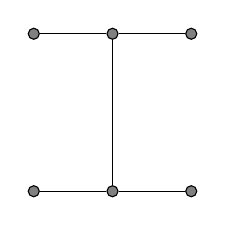
\begin{tikzpicture}[every node/.style={circle, draw, fill=black!50,inner sep=0pt, minimum width=4pt},
            edge_style/.style={draw=black}]
            \node (v1) at (0, 0) {};
            \node (v2) at (1, 0) {};
            \node (v3) at (2, 0) {};
            \node (v4) at (0, 2) {};
            \node (v5) at (1, 2) {};
            \node (v6) at (2, 2) {};
            \draw (v1) edge (v2) {};
            \draw (v2) edge (v3) {};
            \draw (v2) edge (v5) {};
            \draw (v4) edge (v5) {};
            \draw (v5) edge (v6) {};
        \end{tikzpicture}
    \end{subfigure}
    \begin{subfigure}{.25\textwidth}
        \centering
        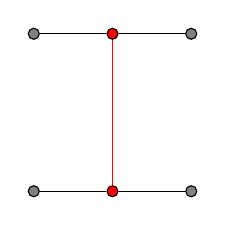
\begin{tikzpicture}[every node/.style={circle, draw, fill=black!50,inner sep=0pt, minimum width=4pt},
            edge_style/.style={draw=black}]
            \tikzset{red edge/.style={draw=red}}
            \tikzset{red node/.style={fill=red}}
            \node (v1) at (0, 0) {};
            \node [red node] (v2) at (1, 0) {};
            \node (v3) at (2, 0) {};
            \node (v4) at (0, 2) {};
            \node [red node] (v5) at (1, 2) {};
            \node (v6) at (2, 2) {};
            \draw (v1) edge (v2) {};
            \draw (v2) edge (v3) {};
            \draw[red edge] (v2) edge (v5) {};
            \draw (v4) edge (v5) {};
            \draw (v5) edge (v6) {};
        \end{tikzpicture}
    \end{subfigure}
    \begin{subfigure}{.24\textwidth}
        \centering
        \begin{tikzpicture}[every node/.style={circle, draw, fill=black!50,inner sep=0pt, minimum width=4pt},
            edge_style/.style={draw=black}]
            \tikzset{green node/.style={fill=green}}
            \node (v1) at (0, 0) {};
            \node (v3) at (2, 0) {};
            \node (v4) at (0, 2) {};
            \node (v6) at (2, 2) {};
            \node [green node] (vn) at (1, 1) {};
            \draw (v1) edge (v2) {};
            \draw (v2) edge (v3) {};
            \draw (v4) edge (v5) {};
            \draw (v5) edge (v6) {};
        \end{tikzpicture}
    \end{subfigure}
    \begin{subfigure}{.24\textwidth}
        \centering
        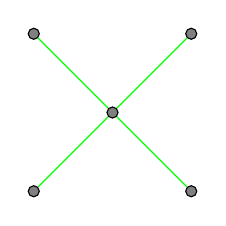
\begin{tikzpicture}[every node/.style={circle, draw, fill=black!50,inner sep=0pt, minimum width=4pt},
            edge_style/.style={draw=black}]
            \tikzset{green edge/.style={draw=green}}
            \node (v1) at (0, 0) {};
            \node (vn) at (1, 1) {};
            \node (v3) at (2, 0) {};
            \node (v4) at (0, 2) {};
            \node (v6) at (2, 2) {};
            \draw [green edge] (v1) edge (vn) {};
            \draw [green edge] (v3) edge (vn) {};
            \draw [green edge] (v4) edge (vn) {};
            \draw [green edge] (v6) edge (vn) {};
        \end{tikzpicture}
    \end{subfigure}
    \caption{Kantenkontaktion an einem Beispiel}
\end{figure}

Hier sehen wir wie einen Kantenkontraktion funktioniert. Und zwar verschmiltz man die beiden, durch die Kante 
verbundenen Knoten zu Einem. Dazu enfernt man zuerst die zu kontrahierende Kante, und ersetzt die beiden Knoten die sie 
verbindet, durch einen neuen Knoten. Danach ersetzt man jede Kante, die zufor mit einem der beiden verschmolzenen Knoten 
verbunden war, durch eine neue, die nun statdessen mit dem neuen Knoten verbunden ist. Betrachten wir nun das Konzept des
Minors:
\begin{definition}[Minor]
    M heißt Minor von G wenn M aus einem Teilgarphen von G, durch Kantenkontaktion hervorgeht.
\end{definition}
So ist zum Beispiel der Dreiecksgraph (a) aus Figur 3 ein Minor des Graphen (b)

\begin{figure}
    \begin{subfigure}{.50\textwidth}
        \centering
        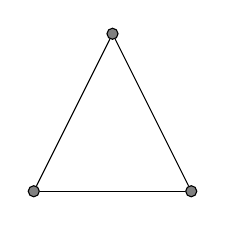
\begin{tikzpicture} [every node/.style={circle, draw, fill=black!50,inner sep=0pt, minimum width=4pt},
            edge_style/.style={draw=black}]
            \node (v1) at (0,0) {};
            \node (v2) at (2,0) {};
            \node (v3) at (1,2) {};
            \draw (v1) edge (v2) {};
            \draw (v2) edge (v3) {};
            \draw (v3) edge (v1) {};
        \end{tikzpicture}
        \caption{}
    \end{subfigure}
    \begin{subfigure}{.48\textwidth}
        \centering
        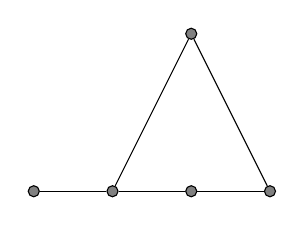
\begin{tikzpicture} [every node/.style={circle, draw, fill=black!50,inner sep=0pt, minimum width=4pt},
            edge_style/.style={draw=black}]
            \node (v1) at (0,0) {};
            \node (v2) at (1,0) {};
            \node (v3) at (2,0) {};
            \node (v4) at (3,0) {};
            \node (v5) at (2,2) {};
            \draw (v1) edge (v2) {};
            \draw (v2) edge (v3) {};
            \draw (v3) edge (v4) {};
            \draw (v4) edge (v5) {};
            \draw (v2) edge (v5) {};
        \end{tikzpicture}
        \caption{}
    \end{subfigure}
    \caption{Minor Beispiel}
\end{figure}
\subsection*{Wichtige Sätze}
Für Planare Graphen gibt es zwei Wichtige Sätze, welche als Voraussetzung für die Funktionalität
des Algorithmus zur Planaritätsbestimmung dienen.
\begin{theorem}{}
    

\end{theorem}

%algo Planaritätsbestimmung (Hopcroft, Tarjan)

\end{document}